\chapter{Towards the \dune{} Near Detector}
\label{chap:dune-nd}

The \AC{} concept, described in Section~\ref{sec:ac_argoncube}, is aimed at enabling a \lartpc{} component in the \dune{} near detector complex.
This chapter will present a more detailed design for the near detector, together with a feasibility study of a \lartpc{} at the expected rates.


\section{\AC{} in the \dune{} Near Detector}
\label{sec:dune-nd_ac}

While Section~\ref{sec:ac_argoncube} gave a general overview of the \AC{} concept, this section focusses on the detailed implementation of the \dune{} near detector.
After the establishment of the key technologies described in this work, the next step will be a \num{2 x 2} module prototype at the university of Bern.
Finally, the current status of an \AC{} \lartpc{} component for the \dune{} near detector complex is given.

\subsection*{\num{2 x 2} Module Prototype}

\begin{figure}[htb]
	\centering
	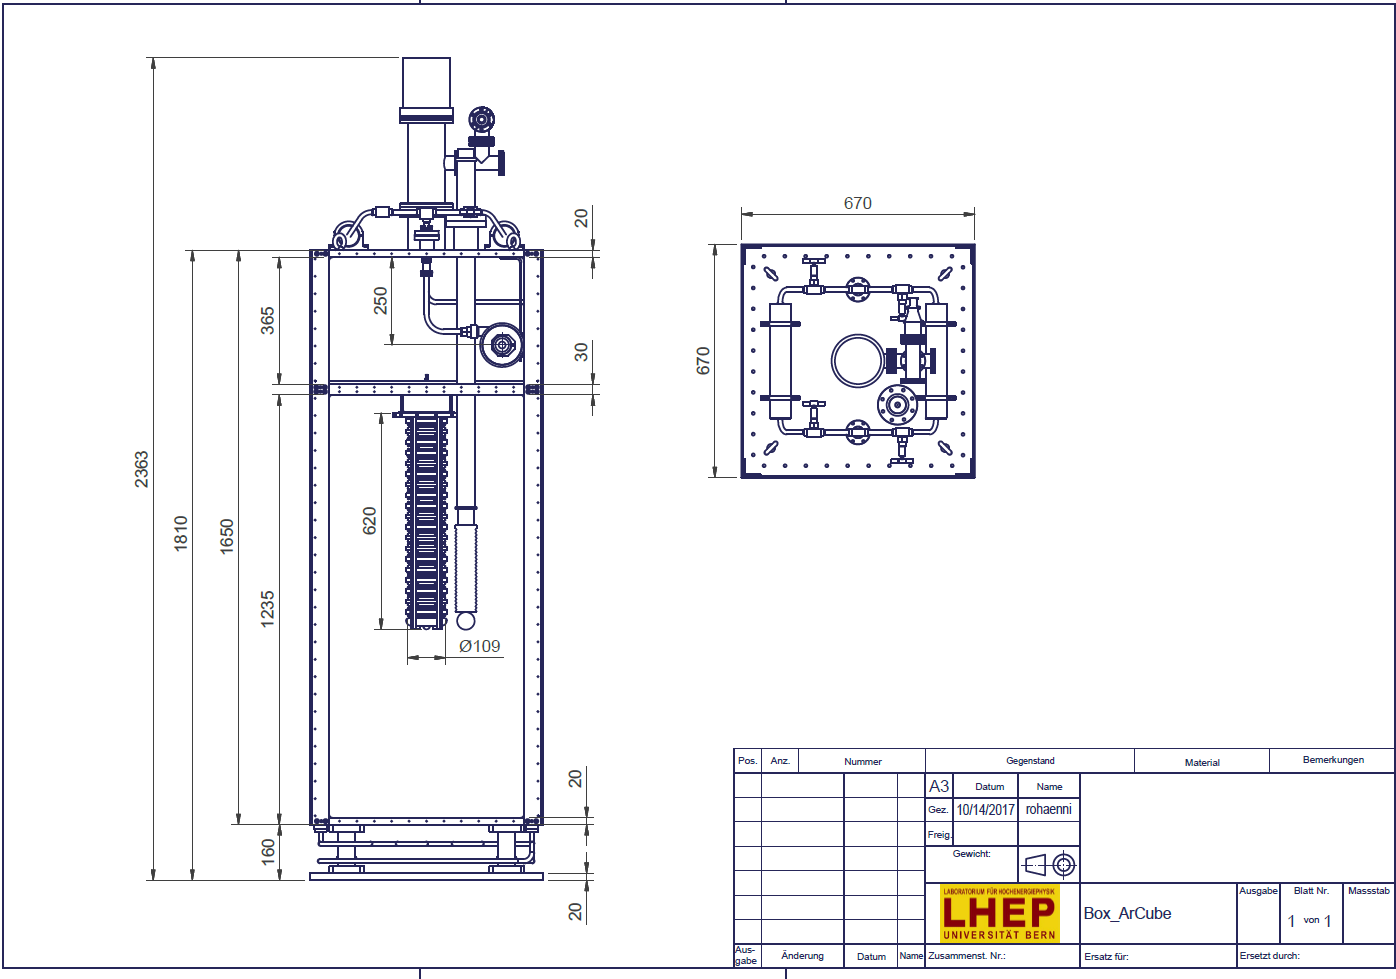
\includegraphics[width=\textwidth]{ac/2x2/dimensions}
	\caption{Dimensions of a \SI{0.67 x 0.67 x 1.81}{\metre} module for the \AC{} \num{2 x 2} module \AC{} prototype at the University of Bern.}
	\label{fig:2x2_dim}
\end{figure}

\begin{figure}[htb]
	\centering
	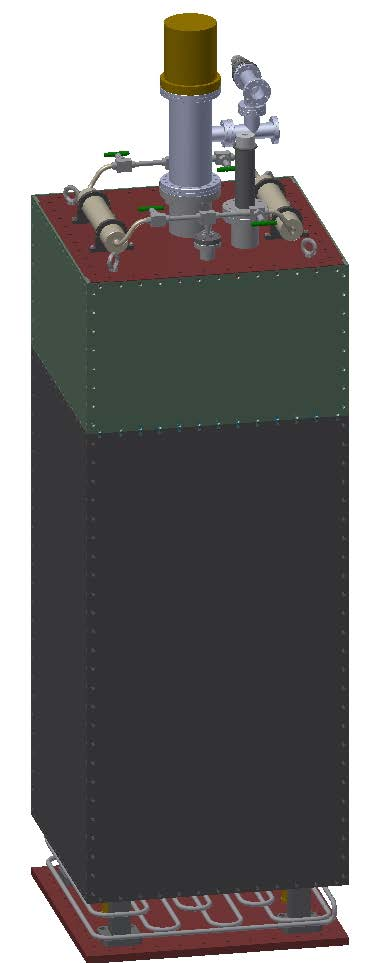
\includegraphics[width=.25\textwidth]{ac/2x2/module_closed}
	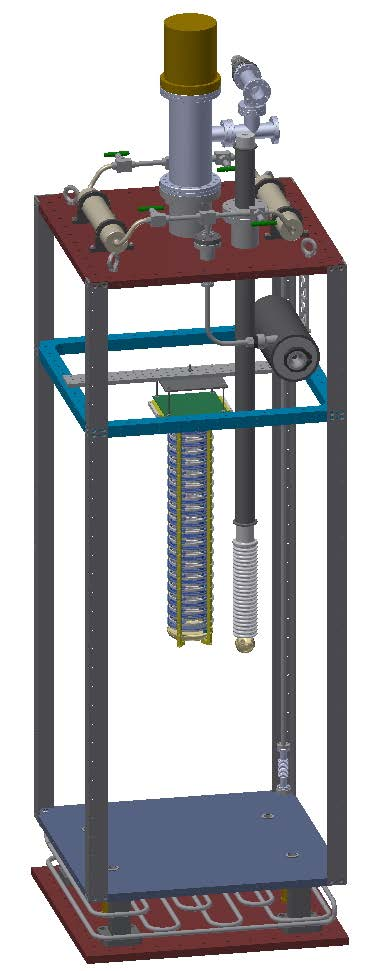
\includegraphics[width=.25\textwidth]{ac/2x2/module_open}
	\caption{Engineering drawing of a \SI{0.67 x 0.67 x 1.81}{\metre} module for the \AC{} \num{2 x 2} module \AC{} prototype at the University of Bern.}
	\label{fig:2x2_mod}
\end{figure}

The four modules will be housed in an existing vacuum-insulated cryostat at the University of Bern.
With its approximately \SI{2.2}{\metre} diameter and \SI{2.8}{\metre} height it provides a \lar{} bath volume of roughly \SI{6}{\metre\cubed}.
To fit inside the bath, the modules are scaled down to a footprint of \SI{0.67 x 0.67}{\metre} and a height of \SI{1.81}{\metre}.
Cooling to the bath is provided by two liquid nitrogen turbo-cooling circuits attached the inner cryostat wall inside the insulation vacuum.
They cool the \lar{} bath via evaporation of the liquid nitrogen.
The nitrogen flow has to be regulated precisely to keep the \lar{} stable and prevent it from boiling or freezing.

The goals of this prototype are testing the mechanical design and cryogenic systems, compare different charge and light readout systems, and study module insertion and extraction procedures with a focus their influence on purity.
For comparison, one of the four modules will be equipped with a classic wire readout.
To investigate purity, first tests will be performed with the \AC{} demonstrator TPC described in Section~\ref{sec:ac_viper}.
The TPC will be mounted inside an otherwise empty module, hanging from the top flange.
This will also serve as a first cryogenic stress-test of the module structure.

The height of the actual TPC in a fully equipped module is \SI{1235}{\milli\metre}.
On the bottom, \SI{160}{\milli\metre} are occupied by the heat exchanger.
The remaining room on top of the TPC is filled up by the HV feedthrough, a buffer gas phase, and a potential recirculation pump.
Everything except for the flanges at the module top and bottom are made from G10, including most of the screws.
The thickness of the side walls is \SI{10}{\milli\metre} while the flanges are made of \SI{20}{\milli\metre} stainless steel plates.
Figure~\ref{fig:2x2_dim} gives the detailed dimensions of a prototype module.
It depicts the first module that will be equipped with the demonstrator TPC.
For this test, an internal pump salvaged from \AT{} will be used in combination with oxygen traps mounted on top of the module.
Engineering drawings of this module are given in Figure~\ref{fig:ac_module}.


\subsection*{Status of the Near Detector Design}

\afterpage{\clearpage}